\section{Event Selection and Categorization}\label{sec:selection}

Signal events are selected on the basis of large values of \ETm and one or more high-\pt jet(s), 
explicitly vetoing isolated leptons and photons. Events are
reconstructed with the CMS detector, following the standard CMS reconstruction~\cite{CMSdetector}. 

The data used for this analysis are collected using either of two triggers designed to record events containing large \ETm. The first requires an \ETm of greater than 120 \gev, calculated only using information from the calorimeter, 
while the second requires an \ETm greater than 95~\gev or 105~\gev, depending on the data-taking period, calculated using  
the particle flow (PF) reconstruction algorithm~\cite{CMS-PAS-PFT-09-001} as well as jet with \pt$>80$ \gev and $|\eta|<2.6$. 
The lowest threshold on the \ETm for the selection of the events is set at 200 \gev in order to maintain a trigger efficiency greater than 
$99$\% with respect to the full event selection. 

Jets are reconstructed from the clustering of PF objects using either the 
anti-$k_{\textrm{T}}$ algorithm~\cite{Cacciari:2008gp} with 0.5 (ak5 jet) as the distance parameter,  
or the Cambridge/Aachen algorithm~\cite{cajets} with 0.8 distance
parameter (ca8). The leading jet is further required to be well
identified, using a standard set of identification criteria~\cite{jec}. The jets are corrected for pileup on the basis of the event energy density and 
proportionally to their area. Data-driven calibrations are then applied to correct the absolute scale of the jet energy~\cite{jec}.

The \ETm is calculated as the magnitude of the negative 
vector sum of the transverse momenta of all final state particles, which are reconstructed 
using the particle-flow (PF) algorithm~\cite{CMS-PAS-PFT-09-001}.
Events with a large mis-reconstructed offline \ETm are removed by applying quality filters. 
The angle between the \ETm and the leading jet in the plane transverse to the beam line, $\Delta\phi$, is required to be larger than 2 to reduce the contribution from multijet QCD events. 
Finally, events are vetoed if they contain at least one well-identified and isolated electron, photon or muon with $p_T>10$~\gev, or a tau with $p_T>15$~\gev.

Selected events are classified into three event categories, based on the topology of the jets, in order to distinguish between 
initial or final state radiation of gluons or quarks and jets arising from hadronic vector boson decays.
The categories are first scrutinized for the presence of an unresolved
vector boson (boosted category), subsequently for a resolved vector
boson (resolved category), and finally the remaining events are collected into the monojet category. 

If the vector boson decays hadronically and has sufficiently high transverse momentum, both its hadronic
decay products are captured by a single reconstructed ``fat''-jet.
Events in the boosted vector boson category are required to
have a reconstructed ca8 jet with $\pt>200$ \gev and  $\ETm>250$ \gev.  Further cuts are applied to improve the vector boson jet
purity by cutting on the variable ``N-subjettiness'' ($\tau_2/\tau_1$ defined in~\cite{Thaler:2010tr,Thaler:2011gf}), which identifies jets with a 
two sub-jet topology, and the pruned jet mass~\cite{Ellis:2009me}. The $\tau_2/\tau_1$ ratio
is required to be smaller than 0.5 and the pruned jet mass, $m_{\mathrm{prune}}$, is selected to
be close to both the W and Z boson masses, namely to satisfy $60<m_{\mathrm{prune}}<110$ \gev.   
Events which contain additional jets close to the ca8 jet, but no closer than $\Delta R < 0.5$,
are selected to include the frequent cases in which initial state radiation yields additional jets. 
If an ak5 jet with $p_T>30$ and $|\eta|<2.5$ is reconstructed, and the opening angle between it 
and the ca8 jet, $\Delta\phi(\mathrm{ak5,ca8})$, is smaller than 2, the event is selected. Events with more than one ak5 jets 
with $p_T>30$ \gev and $|\eta|<2.5$, reconstructed at $\Delta R> 0.5$ with respect to the ca8 jet 
are rejected.
Figure~\ref{fig:boostvtagvars} shows the distributions of $\tau_2/\tau_1$ and $m_{\mathrm{prune}}$, (before the application 
of the jet mass cut) in simulation and data for the boosted event category. Some disagreement is present in the modelling between data and Monte Carlo simulation. This disagreement is well covered by the systematic uncertainties used in the analysis. A detailed discussion of the modelling can be found in ~\cite{Khachatryan:2014vla}.  
\begin{figure*}[hbtp]\begin{center}
\subfigure[]{
 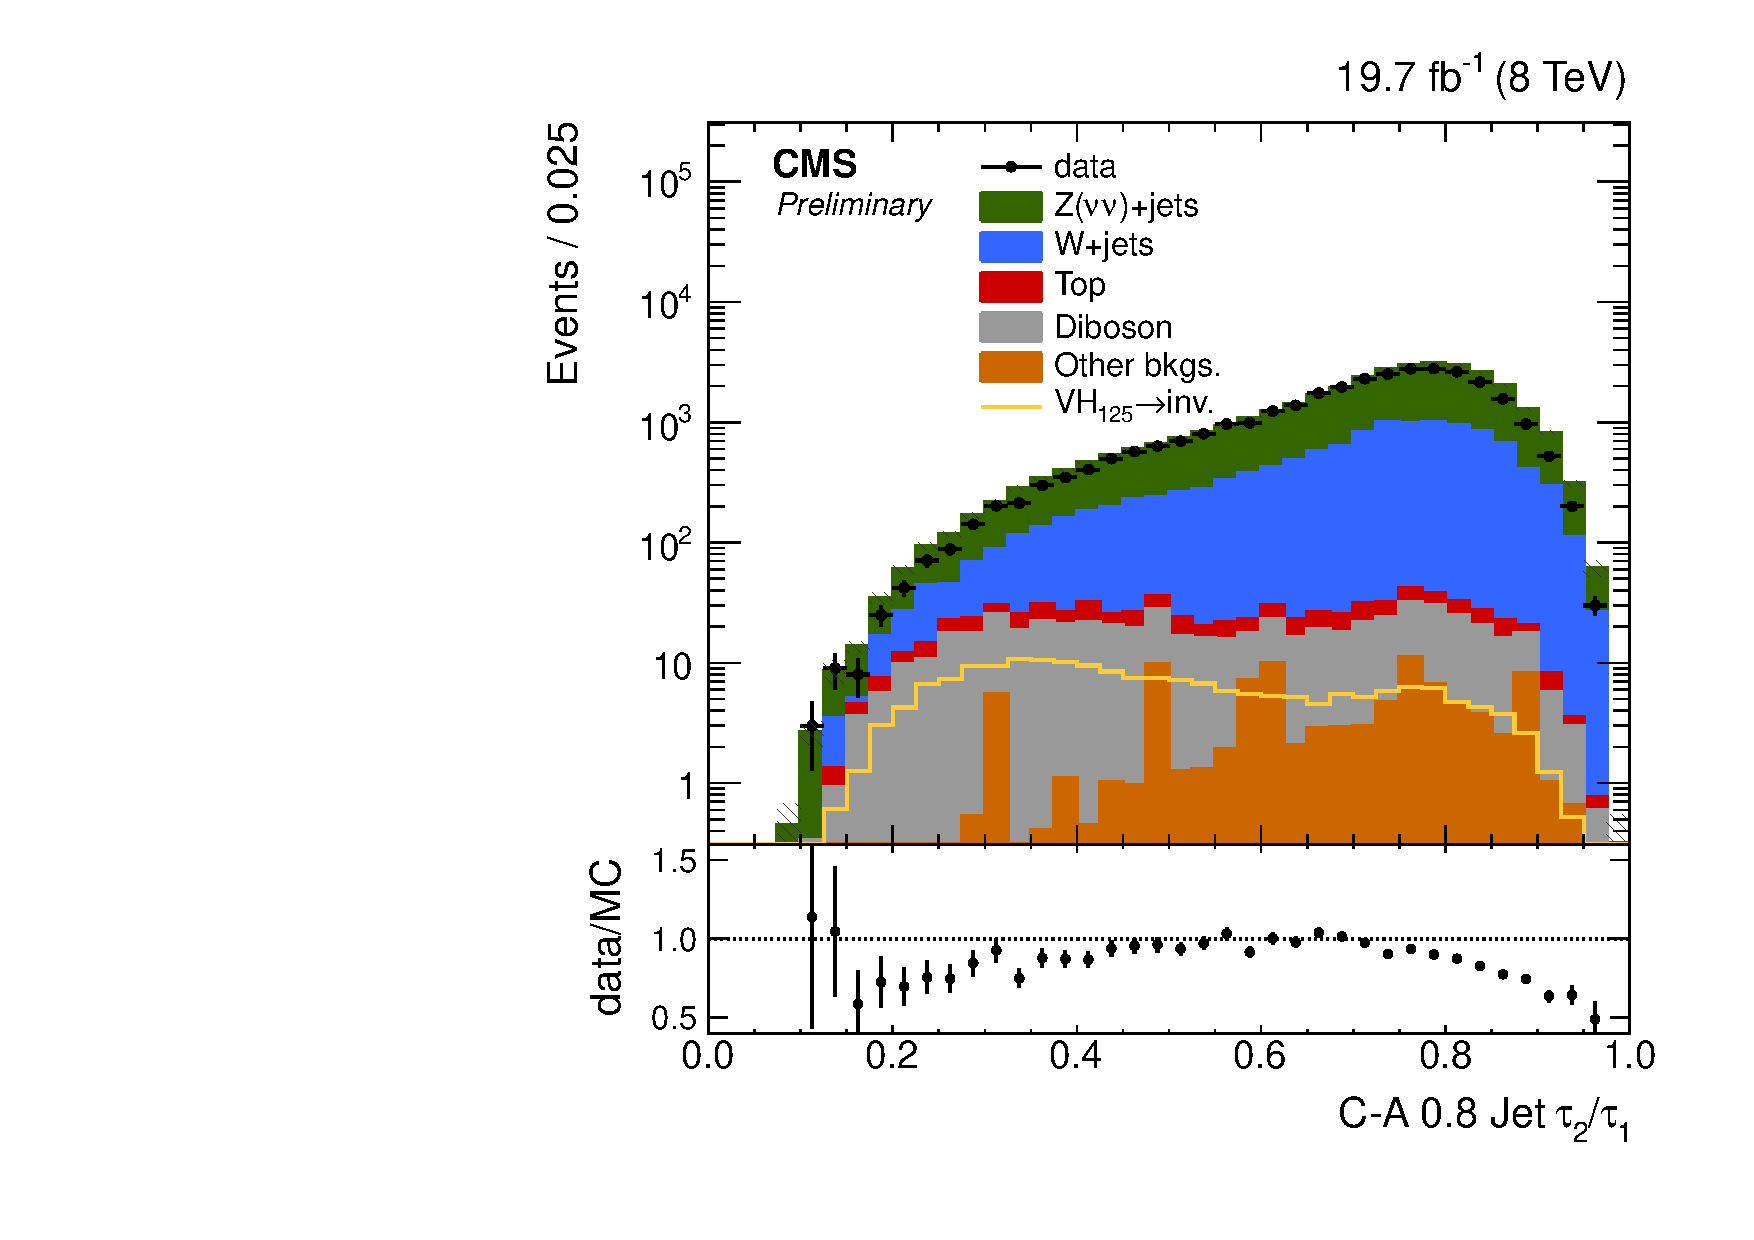
\includegraphics[width=0.49\textwidth]{figures/t2t1_sig_baseline.pdf}
}
\subfigure[]{
 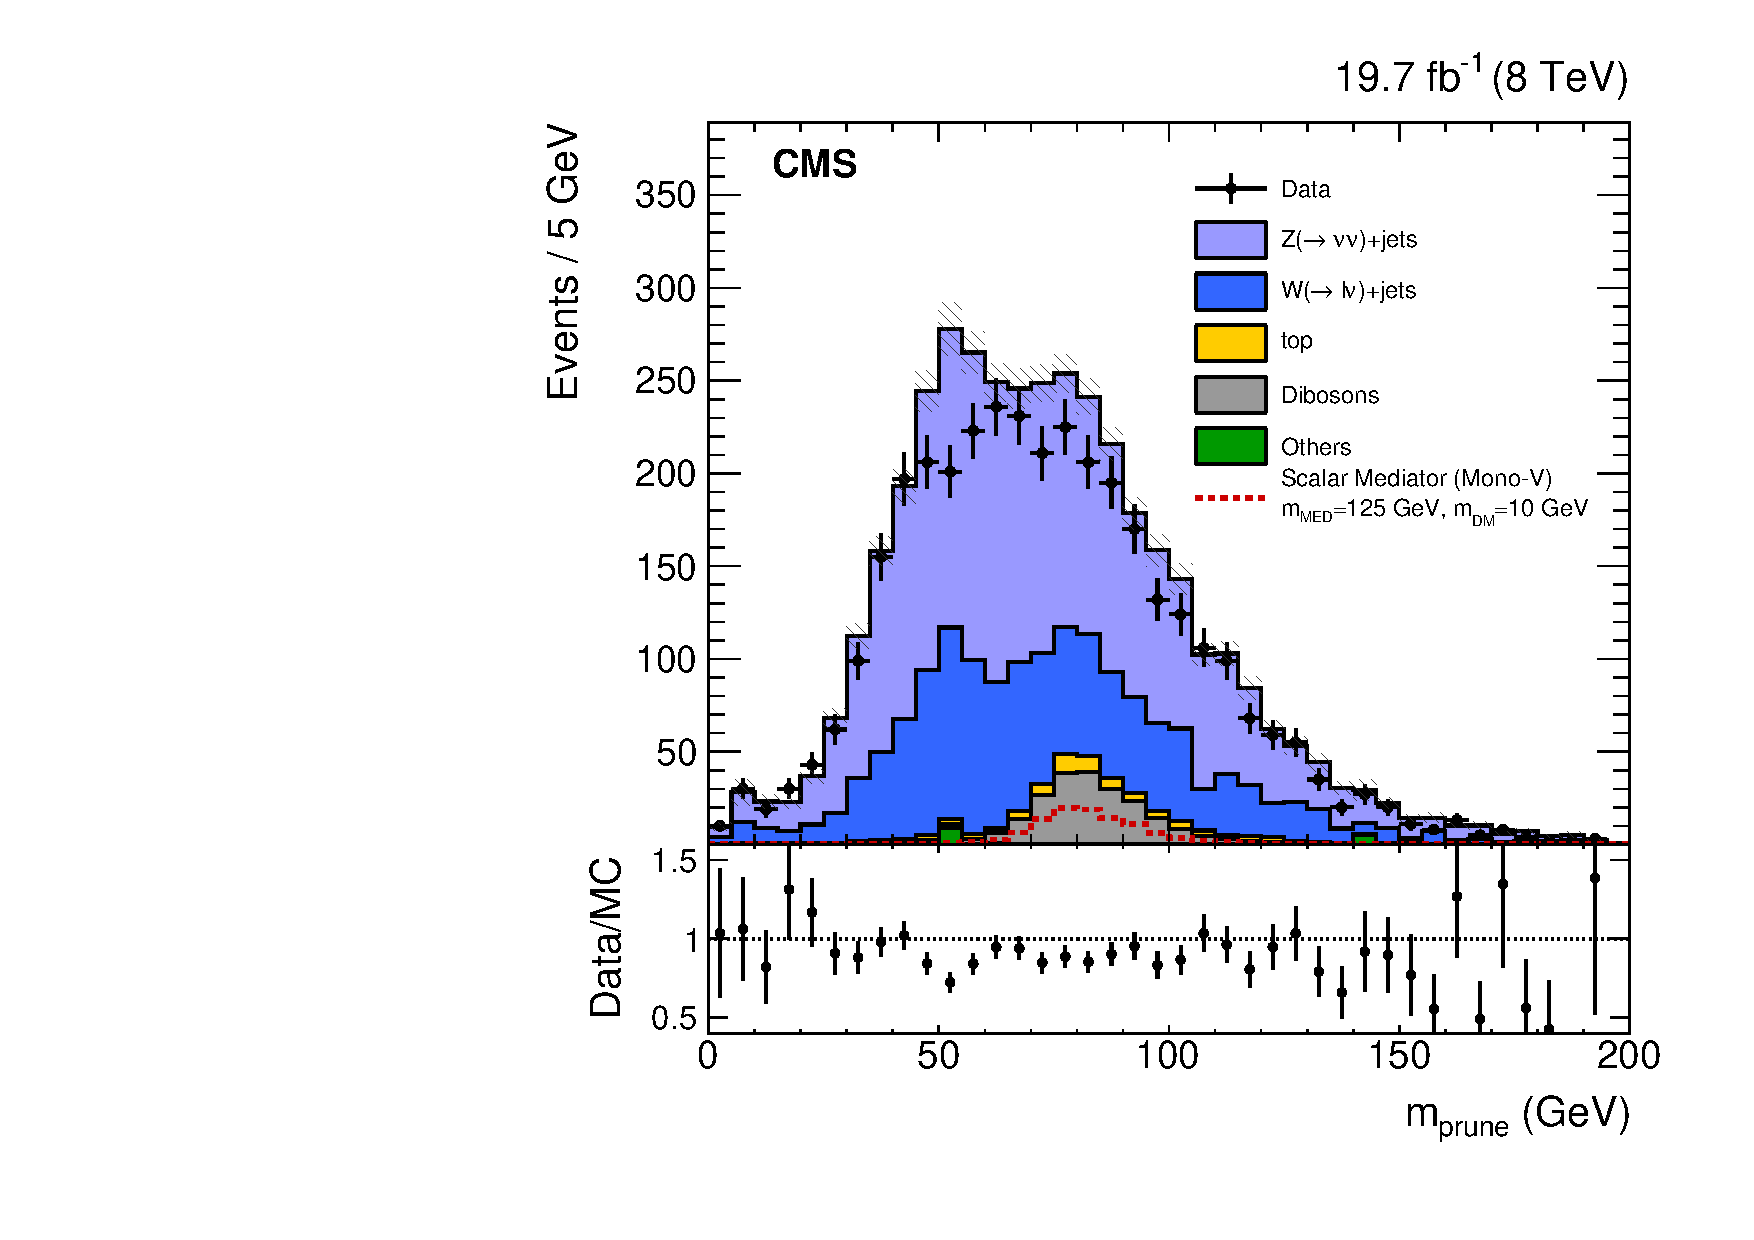
\includegraphics[width=0.49\textwidth]{figures/mass_sig_nomasscut.pdf}
}
 \caption{Distributions of $\tau_2/\tau_1$ before the jet mass cut (a) and pruned jet mass (b) for events in data and MC in the boosted event category. 
 A cut of $\tau_2/\tau_1<$0.5 has been applied in figure b.}
 \label{fig:boostvtagvars}\end{center}\end{figure*}

%\subsection{Resolved V-tagged category}\label{sec:resvtagging}
In cases where the electroweak boson has insufficient transverse momentum for its hadronic
decay to be fully contained in a single reconstructed fat-jet, a selection that looks for decays 
into a pair of ak5 jets is applied to recover the event. 
The selection requires that each jet has $p_T>30$ GeV and $|\eta|<2.5$ and that the dijet has a mass between 60\gev and 110\gev, consistent with originating 
from a W or Z boson. To further reduce the combinatorial background, a
multivariate V-tagger is applied. The inputs to this resolved V-tagger are the values from each jet of likelihood-based discriminator variable 
which distinguishes quark-initiated jets from gluon-initiated
jets~\cite{JME-14-002}, the jet pull angle~\cite{Gallicchio:2010sw}
and the mass drop variable~\cite{Izaguirre:2014ira}. In events 
where multiple dijet pairs are found, the pair with the highest V-tagger value is taken as the candidate. The distribution of the V-tagger variable for SM backgrounds and for a scalar mediator
produced in association with either a W or Z boson is shown in Figure~\ref{fig:vtagger}.
\begin{figure*}[hbtp]\begin{center}
  \subfloat[][]{
 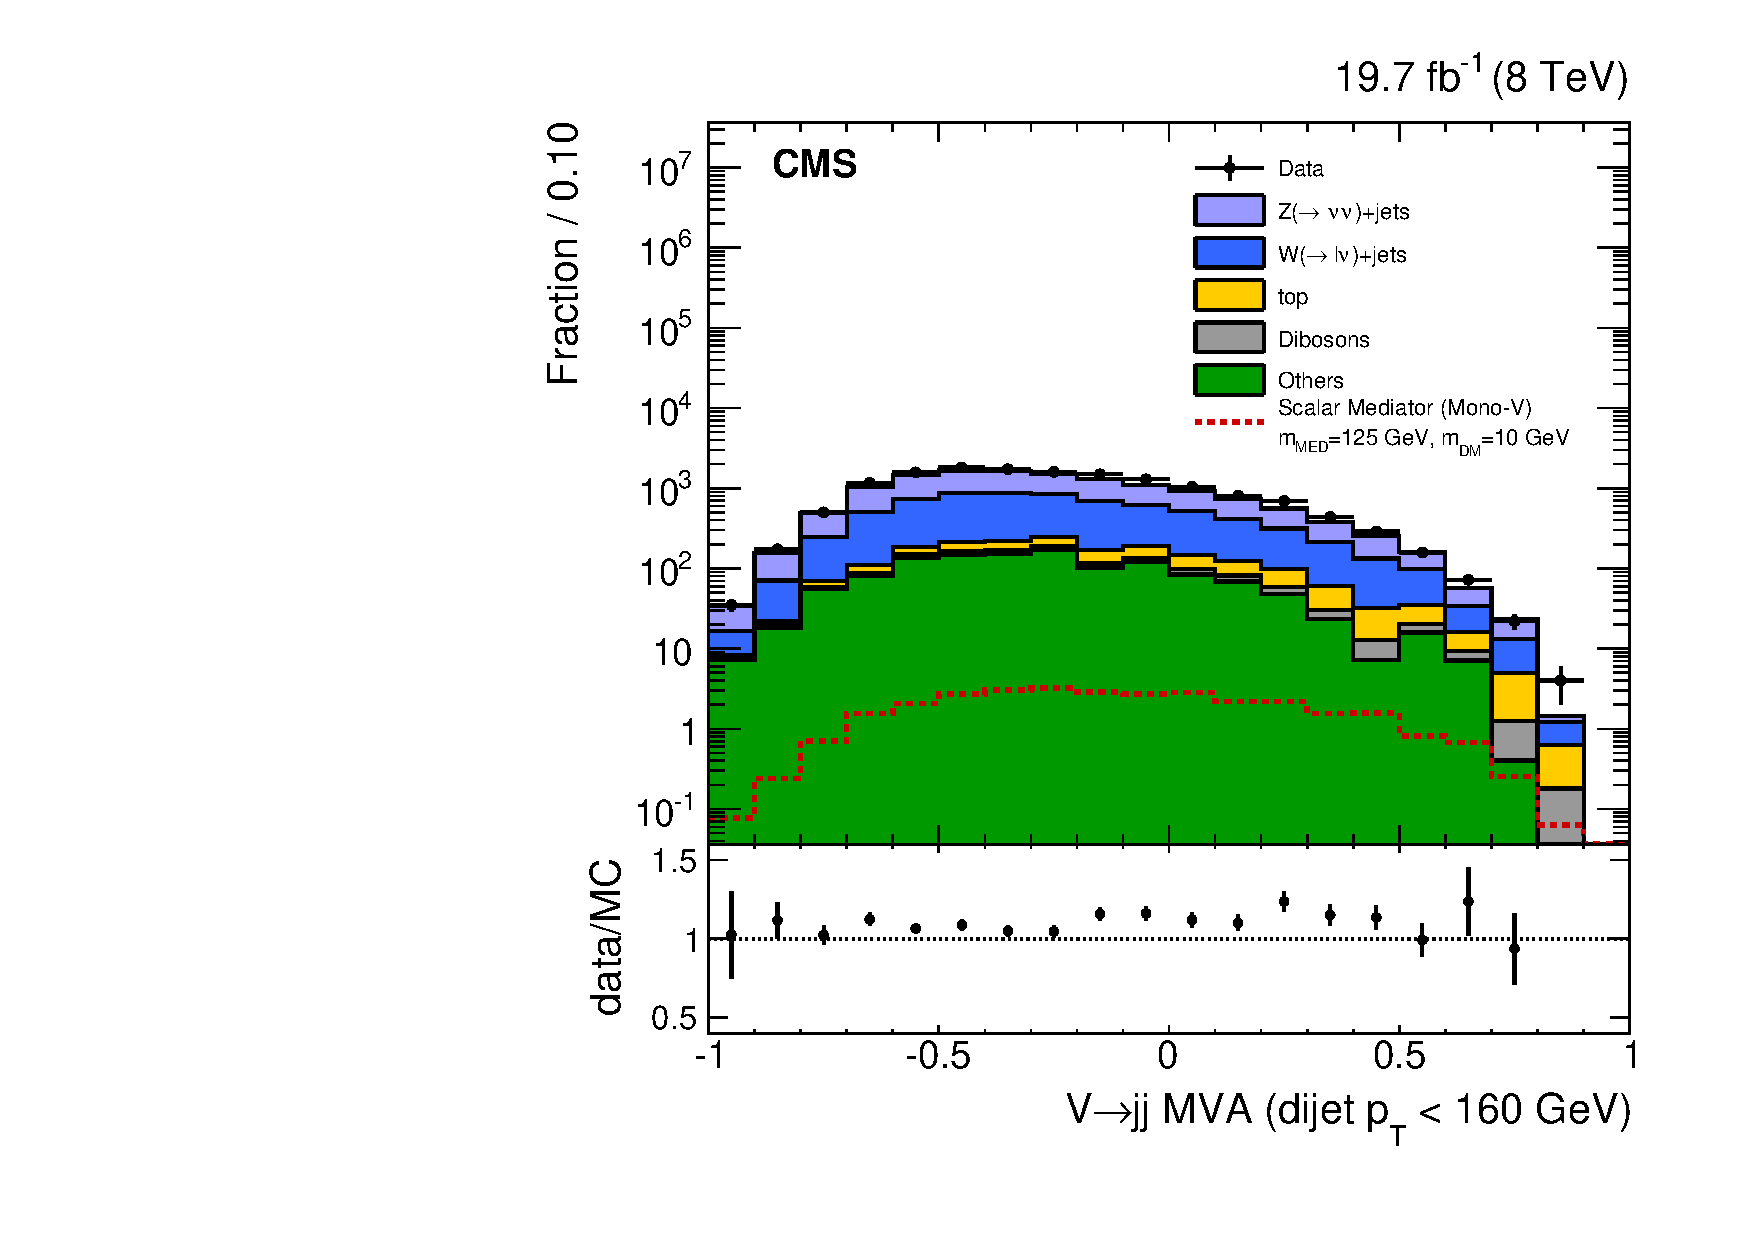
\includegraphics[width=0.49\textwidth]{figures/res_vmvalog_0.pdf}
}
  \subfloat[][]{
 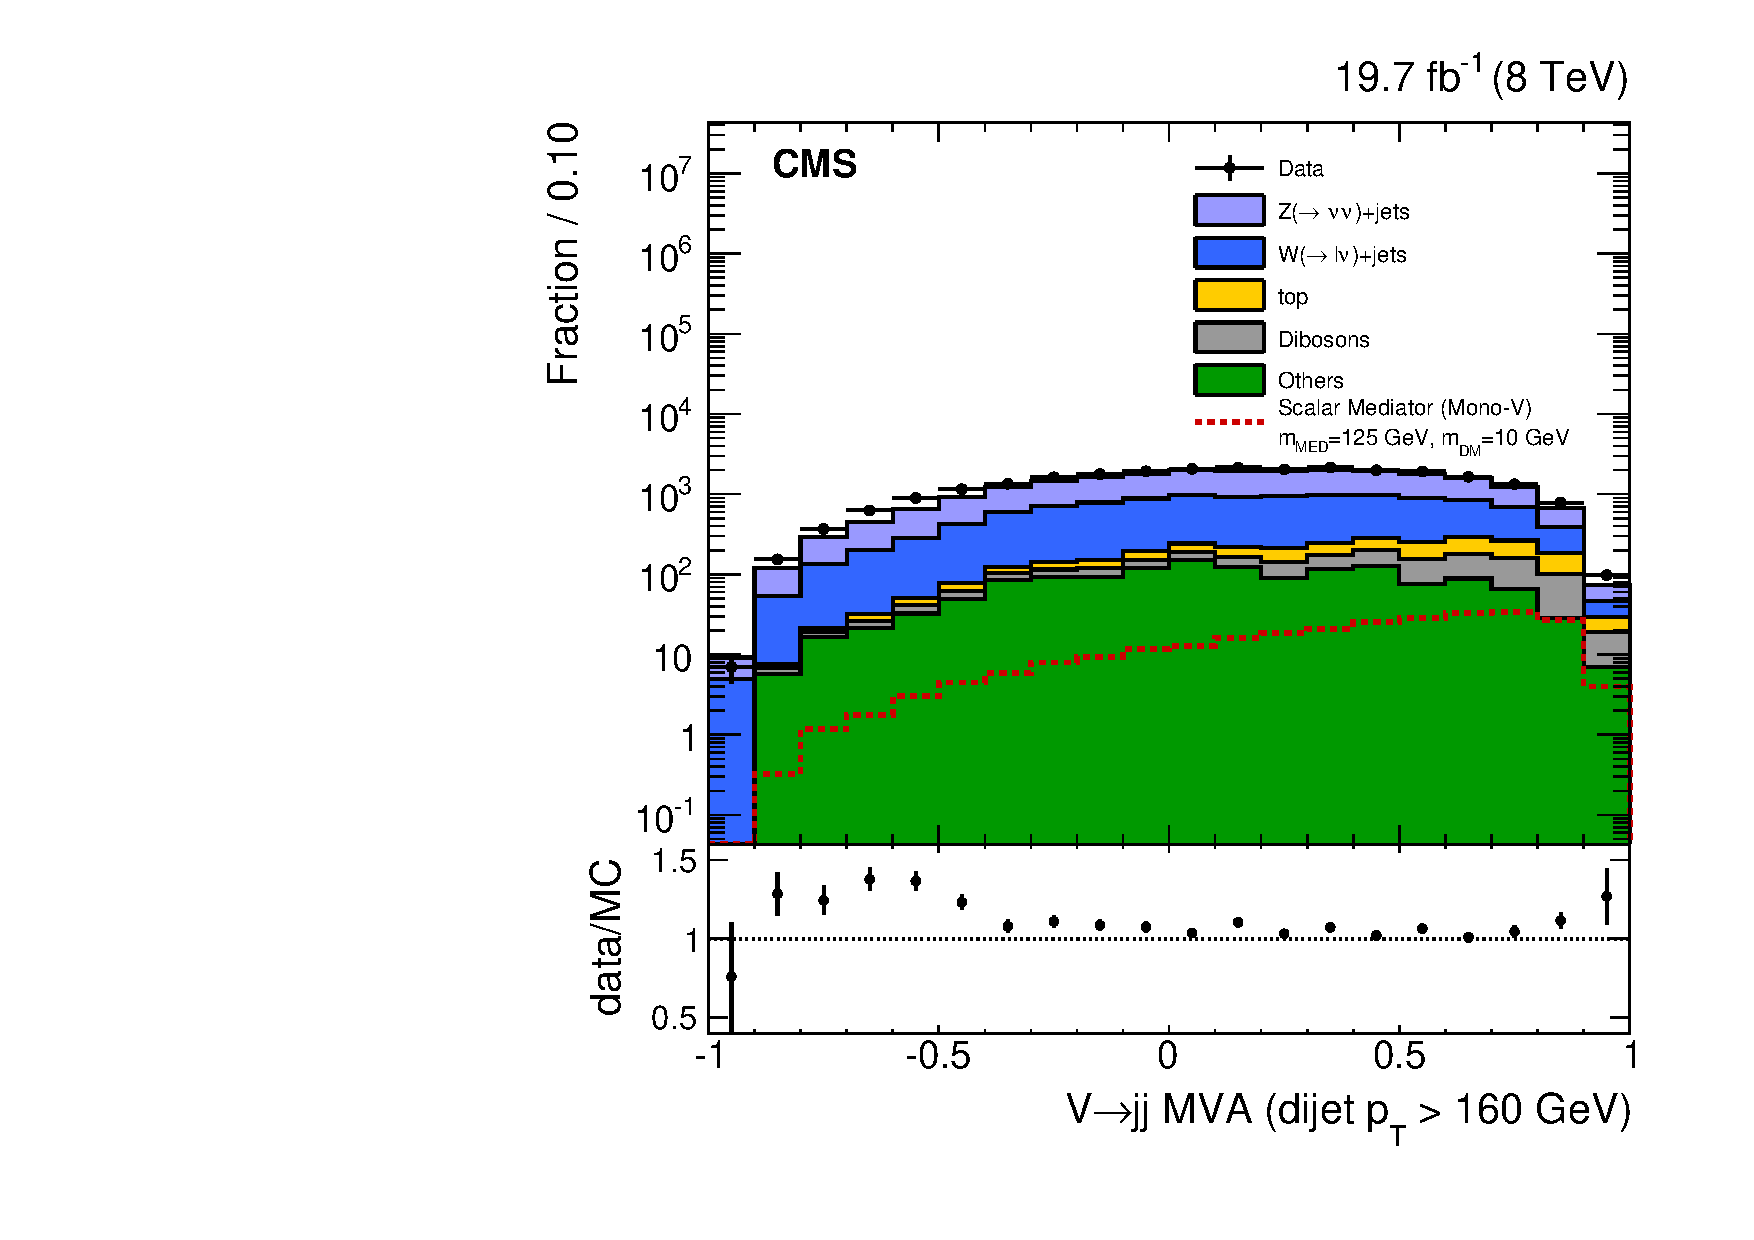
\includegraphics[width=0.49\textwidth]{figures/res_vmvalog_1.pdf}
}
 \caption{
Resolved V-tagger variable distribution in simulation and data after all other
signal region cuts in the resolved category. 
The distributions are shown split into dijet $\pt < 160$ \gev (a) and dijet
$\pt > 160$ \gev (b), corresponding roughly to the point at which jets begin to overlap. 
The expected distribution for the vector boson produced in association with a scalar mediator with is shown.} 
 \label{fig:vtagger}\end{center}\end{figure*}

To reduce contamination from top backgrounds, the event is rejected if it contains a 
b-tagged jet, defined using the CSV medium definition~\cite{BTAG}. Finally, the events are required to 
have $\ETm>250$ \gev. 

The events that do not qualify for either of the two V-tagged categories are required to have a one or two high \pt jets showing characteristics indicative of originating from a \emph{single} quark or gluon. 
For the monojet category, at least one ak5 jet within $|\eta|<2.0$ with \pt greater 
than 150 \gev and a \ETm greater than 200 \gev is required.  
As in the boosted category, events with a second ak5 jet close to the leading one ($\Delta\phi(j_1,j_2) < 2$) 
with $p_T>30$ GeV and $|\eta|<2.5$ are selected to allow the frequent cases where initial state radiation yields two jets.
Events with three or more ak5 jets with $p_T>30$ \gev and $|\eta|<2.5$ are rejected.

To model the expectation from SM backgrounds, simulated samples are produced for the
Z+jets, W+jets, $t\bar{t}$, single-top, and QCD multi-jet processes
using Madgraph~\cite{amcatnlo} interfaced with Pythia6~\cite{Sjostrand:2006za} for hadronization and
fragmentation, where jets from the matrix element are matched to the parton shower following the MLM matching prescription~\cite{Mangano:2006rw}.
Additionally a single-top background sample, produced with
POWHEG~\cite{powheg},  a set of diboson samples, produced directly
with Pythia6, are added. 
The MC samples are corrected to account for the distribution of the number of additional (pileup or PU) interactions
observed in 2012 dataset. Both signal and background samples are additionally corrected to account for the mis-modelling of hadronic recoil in simulation following
the procedure described in~\cite{CMS-PAS-JME-12-002}.


Figure~\ref{fig:ptandmet} shows the \ETm and leading jet $p_{T}$ distributions in data and 
simulation after selection for all three event classes combined. The backgrounds are normalized to 19.7\fbinv 
and the expected distribution for vector mediated DM production assuming a DM mass of 10~\GeV and mediator mass of 1~\TeV is shown. 
The discrepancy between the data and simulation is a result of both mis-modelling of the 
detector resolution and an imperfect theoretical description of the kinematics of the W/Z+jet processes. 
Both effects are corrected for in this analysis using a data-driven approach described in the following section. 

\begin{figure*}[hbtp]\begin{center}
  \subfloat[][]{
 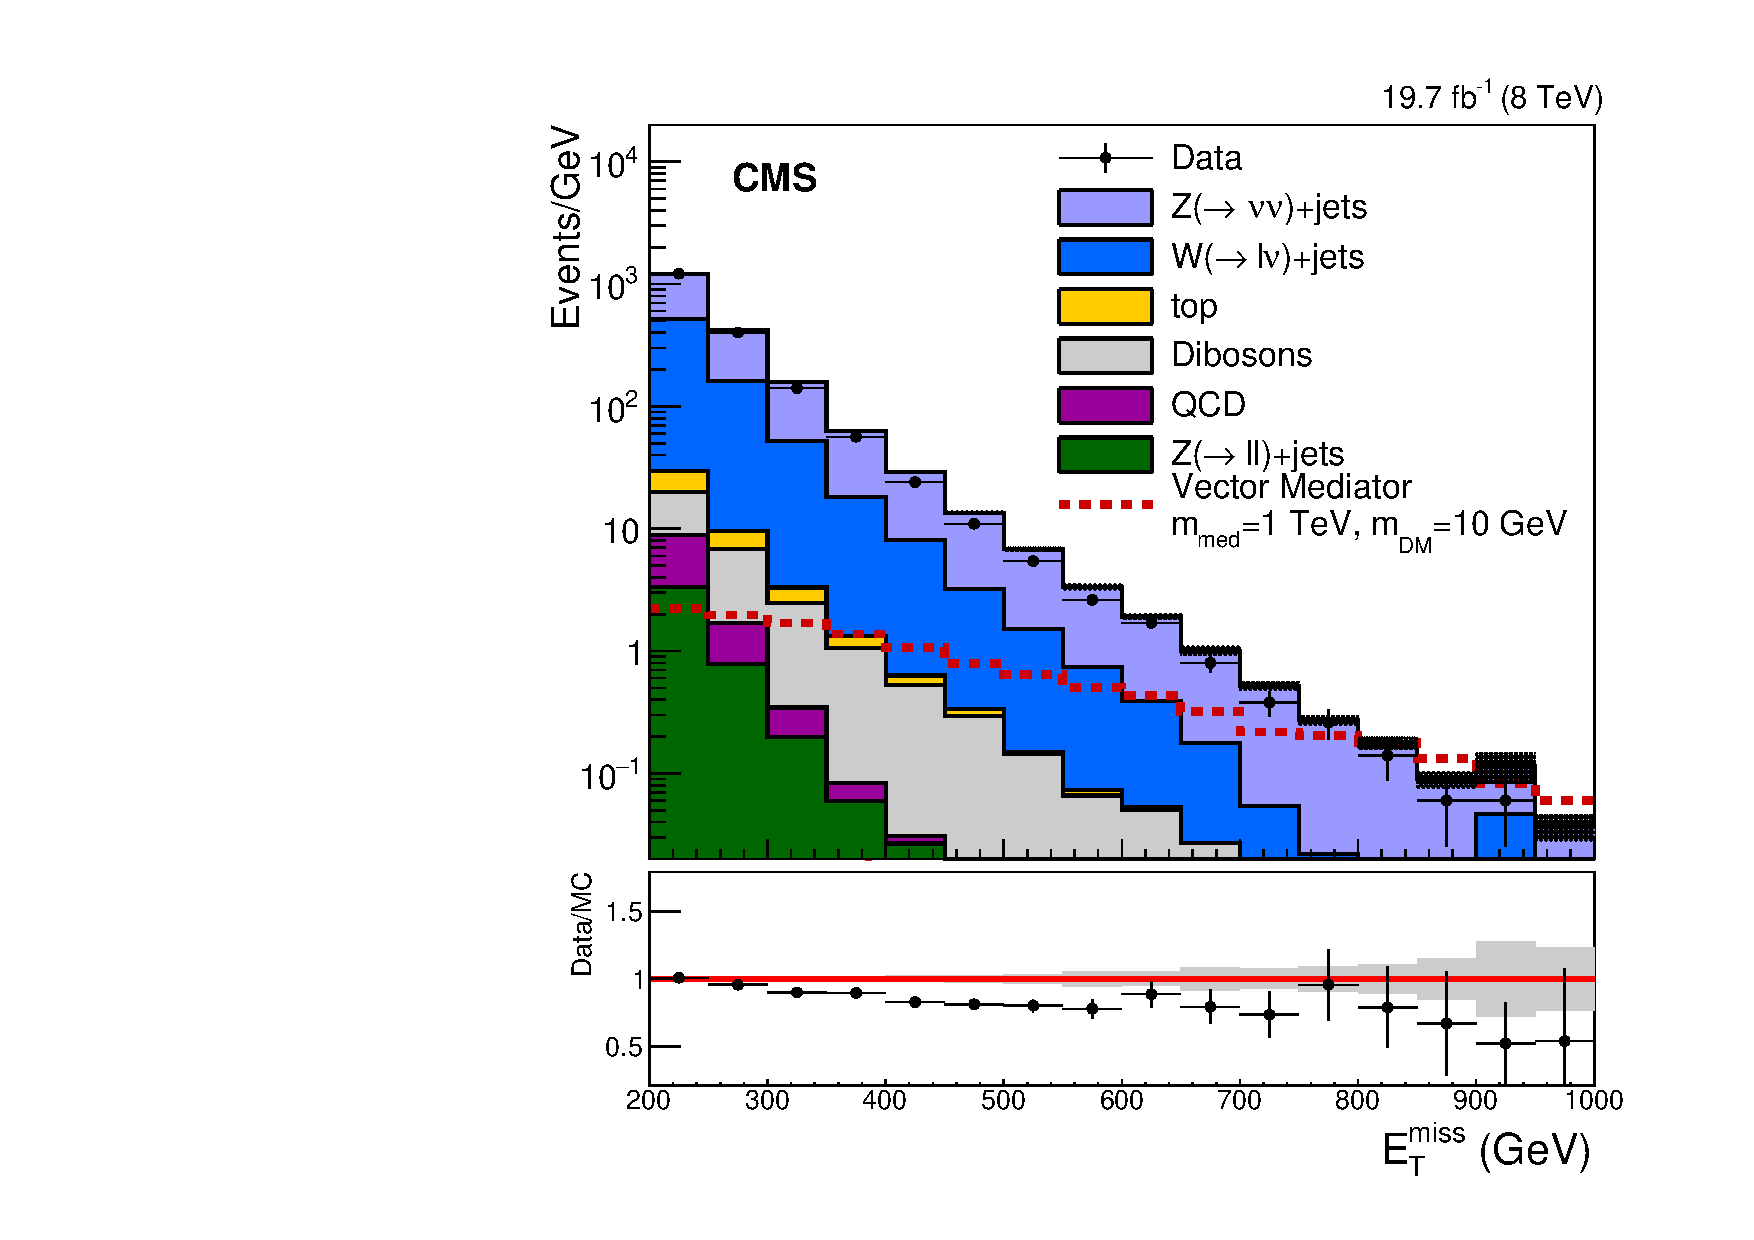
\includegraphics[width=0.49\textwidth]{figures/plot_config_combined_nocorr.pdf}
}
  \subfloat[][]{
 \includegraphics[width=0.49\textwidth]{figures/plot_config_combined_nocorr_jetPT.pdf}\\
}
 \caption{
   Distributions of \ETm (a) and leading jet $p_{T}$ (b) in simulated events and data after the signal selection for all three
   event categories combined. The dashed red line shows the expected distribution assuming vector mediated DM production with $m_{DM}=10$ GeV and $m_{MED}=1$ TeV.
   The gray band in the ratio panels indicate the statistical uncertainty from the limited number of background MC events.
 }
 \label{fig:ptandmet}\end{center}\end{figure*}


